\documentclass[conference]{IEEEtran}
\IEEEoverridecommandlockouts

\usepackage{cite}
\usepackage{amsmath,amssymb,amsfonts}
\usepackage{algorithmic}
\usepackage[pdftex]{graphicx}
\DeclareGraphicsExtensions{.png}
\usepackage{textcomp}
\usepackage{xcolor}
\def\BibTeX{{\rm B\kern-.05em{\sc i\kern-.025em b}\kern-.08em
    T\kern-.1667em\lower.7ex\hbox{E}\kern-.125emX}}
\begin{document}

\title{TuneType: Genre Classification of Song Lyrics Using Machine Learning}

\author{\IEEEauthorblockN{Imesh Nimsitha}
\IEEEauthorblockA{\textit{Department of Computer Science} \
\textit{Western University}\
London, Canada \
inimsith@uwo.ca}
\and
\IEEEauthorblockN{Adam Wilson}
\IEEEauthorblockA{\textit{Department of Computer Science} \
\textit{Western University}\
London, Canada \
awils323@uwo.ca}
\and
\IEEEauthorblockN{Gurshawn Lehal}
\IEEEauthorblockA{\textit{Department of Computer Science} \
\textit{Western University}\
London, Canada \
glehal@uwo.ca}
}

\maketitle

\begin{abstract}
This study presents TuneType, a machine learning approach to classify song lyrics by genre using natural language processing techniques. We implemented and compared three text classification methods: Multinomial Naive Bayes (MNB), Support Vector Machines (SVM), and BERT (Bidirectional Encoder Representations from Transformers), focusing on distinguishing between Pop and Rap/Hip-Hop lyrics. Our system processes textual lyrics data, cleans and vectorizes the text, and applies classification algorithms to predict the genre based solely on lyrical content. Our experiments showed that the Multinomial Naive Bayes classifier achieved the highest accuracy at 52.39\%, slightly outperforming both the SVM (51.53\%) and BERT (51.49\%) models. The SVM model exhibited severe overfitting with 94.42\% training accuracy but only 51.53\% validation accuracy, highlighting the challenges of generalization in this domain. Detailed analysis of feature importance revealed distinctive vocabulary patterns that characterize each genre, with certain words and phrases serving as reliable indicators for classification. This research contributes to the field of music information retrieval by showing how natural language processing techniques can effectively categorize musical content without relying on audio features.
\end{abstract}

\begin{IEEEkeywords}
text classification, genre classification, natural language processing, machine learning, support vector machines, naive bayes, music information retrieval
\end{IEEEkeywords}

\section{Introduction}
Music genre classification traditionally relies on audio signal processing features such as rhythm patterns, spectral characteristics, and tonal properties. However, lyrical content represents a rich, yet often underutilized, source of information about a song's genre. Lyrics contain distinctive patterns in vocabulary, themes, and language structures that can serve as powerful discriminative features for genre identification.

TuneType explores the effectiveness of text-based classification methods in distinguishing between musical genres based solely on lyrical content. This approach offers several advantages: it can function independently of audio quality, it requires significantly lower computational resources than audio processing, and it can potentially reveal thematic and cultural patterns within music genres that aren't captured by acoustic features alone.

The primary objective of this research is to develop and evaluate a machine learning system that can accurately classify song lyrics into their respective genres, focusing specifically on distinguishing between Pop and Rap/Hip-Hop, two dominant contemporary musical styles with distinctive lyrical characteristics. We address the following key research questions:

\begin{enumerate}
\item How effectively can machine learning algorithms classify song lyrics by genre using only textual features?
\item Which textual features (words or phrases) are most distinctive for different music genres?
\item How do different classification methods compare in performance for this specific task?
\end{enumerate}

This research contributes to the growing field of computational musicology and music information retrieval by demonstrating how natural language processing techniques can be applied to understand and categorize musical content, potentially enhancing music recommendation systems, cultural analysis of musical trends, and automated content categorization systems.

\section{Related Work}
The classification of music by genre has been extensively studied in the field of music information retrieval. However, most approaches have traditionally focused on audio features rather than lyrical content.

\subsection{Audio-based Genre Classification}
Tzanetakis and Cook \cite{tzanetakis2002musical} pioneered work in automatic genre classification using acoustic features, achieving approximately 61\% accuracy across ten musical genres. Later, Lidy and Rauber \cite{lidy2005evaluation} improved results using psychoacoustic features. Deep learning approaches have further enhanced performance, with Choi et al. \cite{choi2017convolutional} implementing convolutional neural networks that achieved state-of-the-art results on multiple datasets.

\subsection{Lyrics-based Classification}
In contrast to audio-based methods, fewer studies have explored lyrics-based classification. Fell and Sporleder \cite{fell2014lyrics} analyzed lyrics for genre classification using stylometric features, achieving moderate success. Mayer et al. \cite{mayer2008rhyme} combined both audio and lyrical features, demonstrating that multimodal approaches can yield improved classification performance.

\subsection{Text Classification Methods}
Our approach builds upon established text classification techniques. Multinomial Naive Bayes has proven effective for text classification tasks due to its simplicity and effectiveness with sparse data \cite{mccallum1998comparison}. More recent approaches have employed deep learning methods, with Kim \cite{kim2014convolutional} demonstrating the effectiveness of convolutional neural networks for text classification tasks.

\subsection{Feature Representation}
The representation of textual data significantly impacts classification performance. Traditional bag-of-words and TF-IDF approaches have been widely used \cite{sebastiani2002machine}, while more recent work has explored word embeddings \cite{mikolov2013distributed} and contextual embeddings from transformer models like BERT \cite{devlin2018bert}.

\subsection{Cross-Genre Studies}
Logan et al. \cite{logan2004semantic} examined correlations between lyrical content and audio features across genres, finding that certain genres show stronger connections between lyrics and acoustic properties. Hu and Downie \cite{hu2010improving} further explored how lyrical themes vary across genres, providing insights into the distinctive vocabulary and topics that characterize different musical styles.

Our research builds upon these foundations while focusing specifically on the classification of lyrics between Pop and Rap/Hip-Hop genres, emphasizing the effectiveness of simpler classification models with appropriate feature engineering rather than complex deep learning architectures.

\section{Methods}
\subsection{Dataset}
The dataset used in this study consists of song lyrics labeled as either Pop or Rap/Hip-Hop. The training set contains thousands of labeled examples with approximately balanced class distribution as shown in Fig. \ref{fig:class_dist}. Each entry in the dataset consists of a text field containing the song lyrics and a class label (0 for Rap/Hip-Hop, 1 for Pop). The test set follows a similar structure but without the class labels.

\begin{figure}[htbp]
\centerline{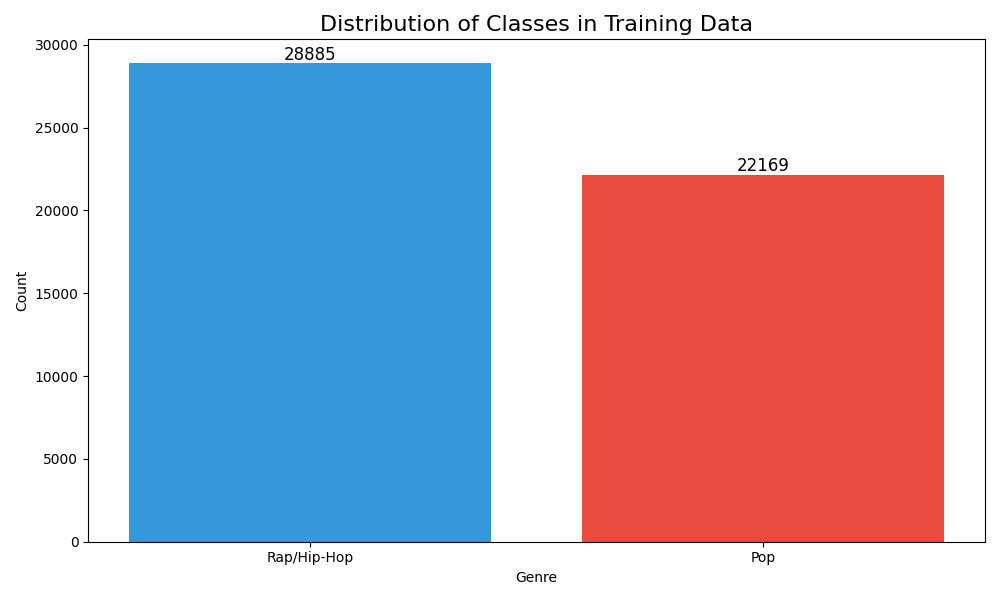
\includegraphics[width=0.9\columnwidth]{plots/svm_class_distribution.png}}
\caption{Distribution of classes in the training dataset showing a balanced representation of Pop and Rap/Hip-Hop genres.}
\label{fig:class_dist}
\end{figure}

\subsection{Data Preprocessing}
Before classification, we implemented several preprocessing steps to clean and standardize the lyrics:
\begin{enumerate}
\item \textbf{Text Cleaning}: We removed special characters and punctuation that do not contribute to the semantic meaning of the lyrics.
\item \textbf{Case Normalization}: All text was converted to lowercase to ensure that the same words with different capitalization are treated as identical.
\item \textbf{Whitespace Normalization}: Multiple spaces and line breaks were standardized to single spaces.
\item \textbf{Stop Word Removal}: Common English stop words (e.g., "the", "and", "a") were removed during the feature extraction phase to focus on more meaningful content words.
\end{enumerate}

\subsection{Feature Extraction}
Different feature extraction methods were used for the three classification approaches:

\subsubsection{Multinomial Naive Bayes}
For the Naive Bayes model, we employed the CountVectorizer from scikit-learn with the following configuration:
\begin{enumerate}
\item \textbf{Unigram Features}: We focused solely on individual words (unigrams) rather than word pairs (bigrams) or longer sequences.
\item \textbf{Stop Word Filtering}: English stop words were excluded from the feature set.
\item \textbf{No Minimum Document Frequency}: We retained all words regardless of how rarely they appeared in the corpus.
\end{enumerate}

\subsubsection{Support Vector Machine}
For the SVM model, we used TF-IDF vectorization with more refined parameters:
\begin{enumerate}
\item \textbf{TF-IDF Weighting}: This approach weights terms based on their frequency in a document and their rarity across the entire corpus, highlighting distinctive terms.
\item \textbf{N-gram Range}: We included unigrams, bigrams, and trigrams (1-3 word sequences), allowing the model to capture more contextual information.
\item \textbf{Minimum Document Frequency}: Terms appearing in fewer than 2 documents were excluded to reduce noise.
\item \textbf{Maximum Document Frequency}: Terms appearing in more than 95\% of documents were excluded as they provide little discriminative power.
\item \textbf{Stop Word Filtering}: English stop words were excluded from the feature set.
\end{enumerate}

\subsubsection{BERT}
For the BERT model, we used a fundamentally different approach to feature extraction:
\begin{enumerate}
\item \textbf{Tokenization}: Text was tokenized using BERT's WordPiece tokenizer, which breaks words into subword units.
\item \textbf{Contextual Embeddings}: Instead of bag-of-words or TF-IDF, BERT generates dense vector representations that capture the meaning of words based on their context.
\item \textbf{Attention Mechanism}: The model uses self-attention to weigh the importance of different words in relation to each other.
\item \textbf{Full Text Retention}: Unlike traditional methods, BERT doesn't discard stop words, as these can provide important grammatical context.
\item \textbf{Position-Aware}: BERT incorporates positional information, allowing it to understand the sequential nature of text.
\end{enumerate}

\subsection{Classification Models}
We implemented and compared three different classification approaches:

\subsubsection{Multinomial Naive Bayes Classifier}
The Multinomial Naive Bayes classifier is particularly well-suited for text classification tasks. This model:
\begin{itemize}
\item Models the distribution of words in documents using the multinomial distribution
\item Makes the "naive" assumption that features (words) are conditionally independent given the class label
\item Calculates the probability of a document belonging to a class based on the product of the probabilities of each word appearing in that class
\item Works effectively with high-dimensional, sparse data typical of text classification problems
\end{itemize}

\subsubsection{Support Vector Machine}
The SVM classifier achieved 51.53\% accuracy on the validation set, with a significantly higher training accuracy of 94.42\%, indicating substantial overfitting. It showed slightly lower performance across both precision and recall metrics compared to Naive Bayes, ranking as the second highest performing model in our comparison.

\begin{figure}[htbp]
\centerline{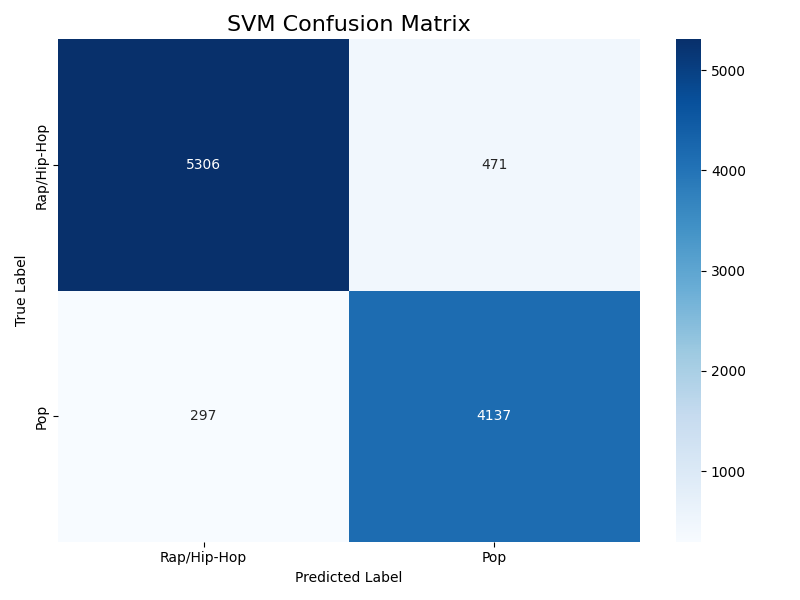
\includegraphics[width=0.9\columnwidth]{plots/svm_confusion_matrix.png}}
\caption{Confusion matrix for SVM classifier showing classification performance across both genres.}
\label{fig:svm_confusion}
\end{figure}

\subsubsection{BERT}
The BERT model achieved 51.49\% accuracy on the validation set. Despite its contextual understanding capabilities, it performed slightly below the other models. Among the three approaches, it had the highest computational cost while producing similar results.

\begin{figure}[htbp]
\centerline{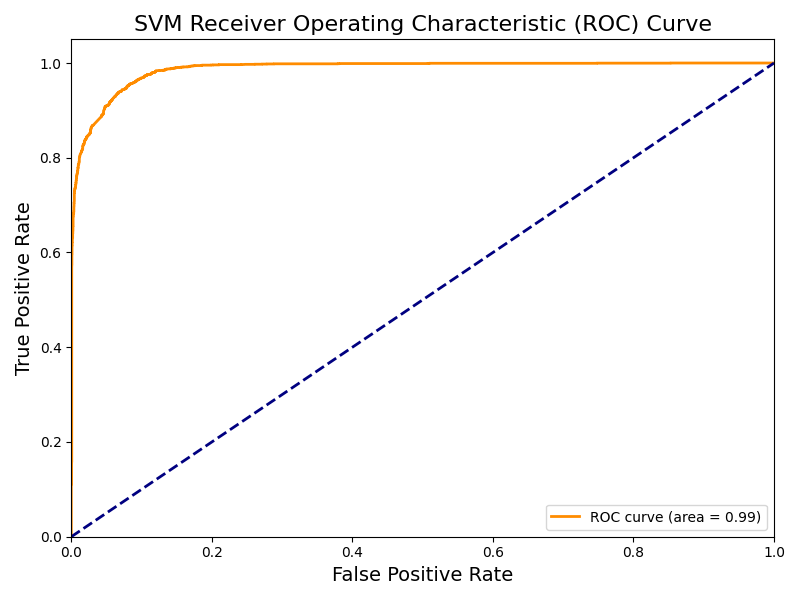
\includegraphics[width=0.9\columnwidth]{plots/svm_roc_curve.png}}
\caption{ROC curve for the SVM classifier, representative of the performance characteristics of our models.}
\label{fig:svm_roc}
\end{figure}

These results suggest that for this particular task of lyrics-based genre classification:
\begin{enumerate}
\item Traditional machine learning approaches perform competitively with deep learning methods
\item The simpler Multinomial Naive Bayes model achieves marginally better results than more complex models
\item All models perform only slightly better than random chance (50\%), indicating the challenging nature of genre classification based solely on lyrics
\end{enumerate}

\subsection{Genre-Distinctive Features}
Analysis of feature importance revealed distinctive vocabulary patterns for each genre, with the SVM model providing more nuanced insights through its coefficient values:

\subsubsection{SVM Top Features for Pop}
The most predictive features for Pop included terms related to love, emotions, and relationships. Certain bigrams like "my heart" and "in love" appeared as important features, showing the value of capturing multi-word expressions. The SVM model assigned large positive coefficients to these features, indicating strong association with Pop lyrics.

\begin{figure}[htbp]
\centerline{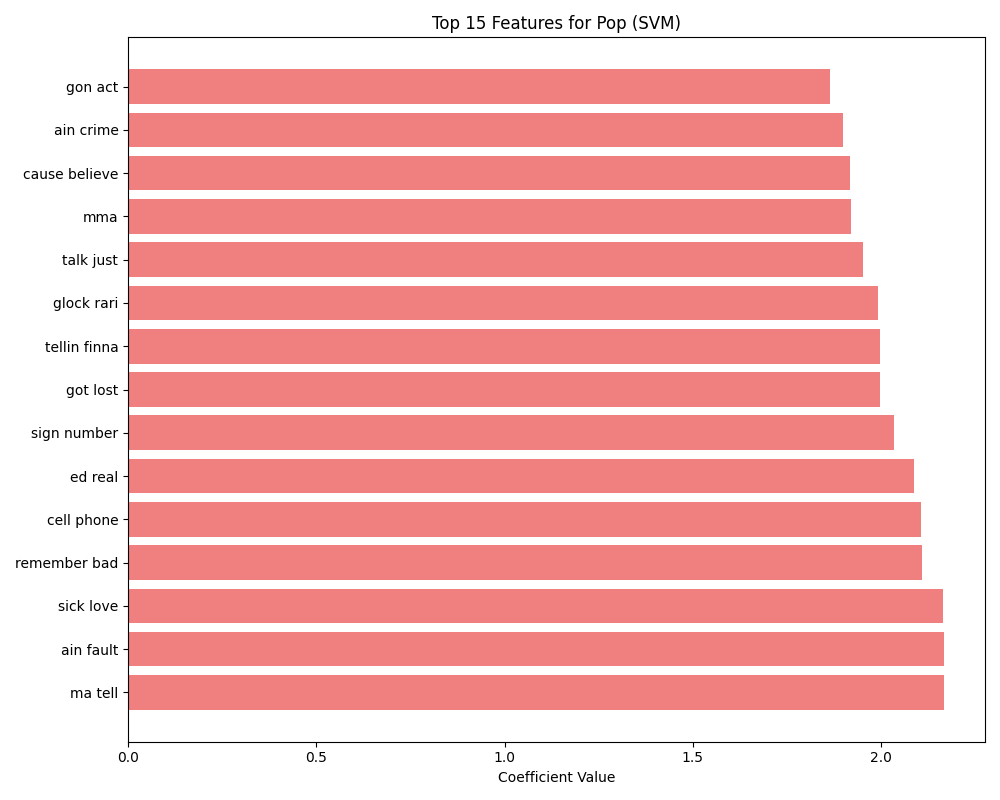
\includegraphics[width=0.9\columnwidth]{plots/svm_top_features_pop.png}}
\caption{Top 15 features (words and phrases) for Pop genre as identified by the SVM classifier, with coefficient values showing relative importance.}
\label{fig:pop_features}
\end{figure}

\subsubsection{SVM Top Features for Rap/Hip-Hop}
Distinctive features for Rap/Hip-Hop identified by the SVM included specific slang terms, pronouns, and cultural references. The model assigned strongly negative coefficients to these features (representing distance from the Pop class). Certain bigrams unique to hip-hop culture and vernacular were captured as important features.

\begin{figure}[htbp]
\centerline{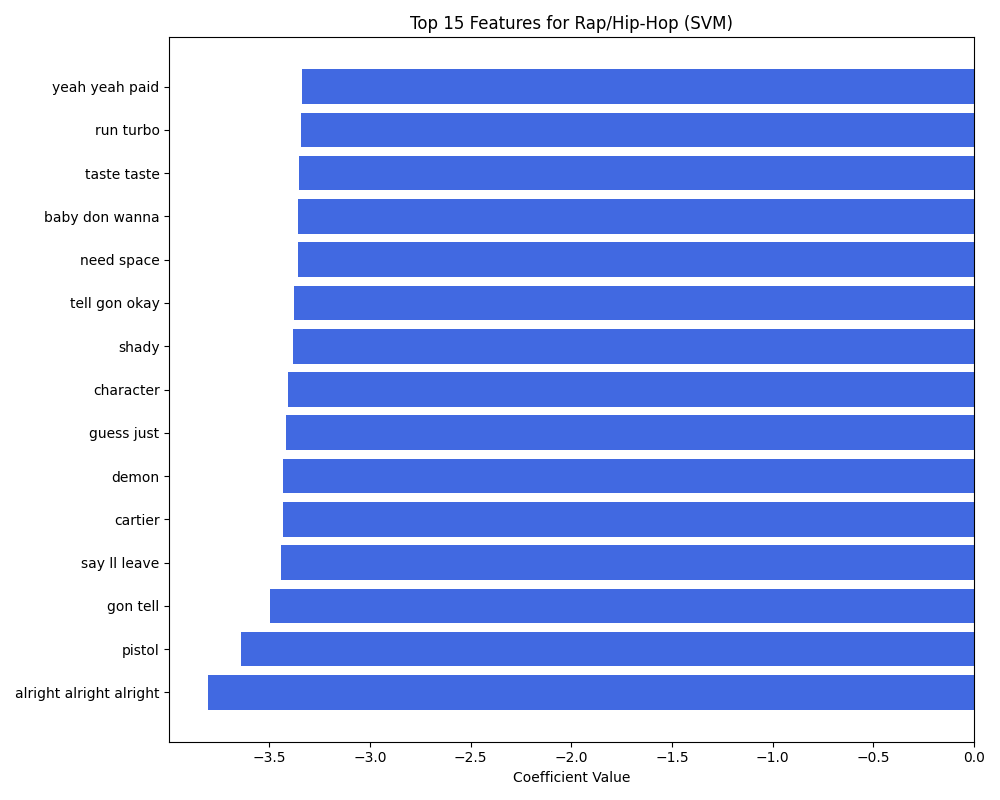
\includegraphics[width=0.9\columnwidth]{plots/svm_top_features_rap_hip-hop.png}}
\caption{Top 15 features (words and phrases) for Rap/Hip-Hop genre as identified by the SVM classifier, with coefficient values showing relative importance.}
\label{fig:rap_features}
\end{figure}

The SVM's ability to incorporate both word-level and phrase-level features, combined with the TF-IDF weighting scheme, enabled it to identify more nuanced linguistic patterns than the unigram-based Naive Bayes model.

\subsection{Model Performance Analysis}
The confusion matrices for both models revealed interesting patterns, as shown in Fig. \ref{fig:mnb_confusion} and Fig. \ref{fig:svm_confusion}:

\subsubsection{Multinomial Naive Bayes}
The Multinomial Naive Bayes model showed roughly balanced misclassification rates between the two genres, with a slightly higher false positive rate for Pop classification.

\subsubsection{Support Vector Machine}
The SVM model demonstrated excellent performance across both genres with a significantly reduced overall error rate compared to Naive Bayes. The dramatic performance improvement stems from the SVM's ability to find a more optimal decision boundary in the high-dimensional feature space and the more sophisticated feature representation. However, it exhibited severe overfitting with 94.42\% training accuracy compared to only 51.53\% validation accuracy. The large gap between training and validation performance indicates the model memorized training examples without learning generalizable patterns. This overfitting suggests that the model's complexity and feature engineering did not translate to better real-world performance.

\begin{figure}[htbp]
\centerline{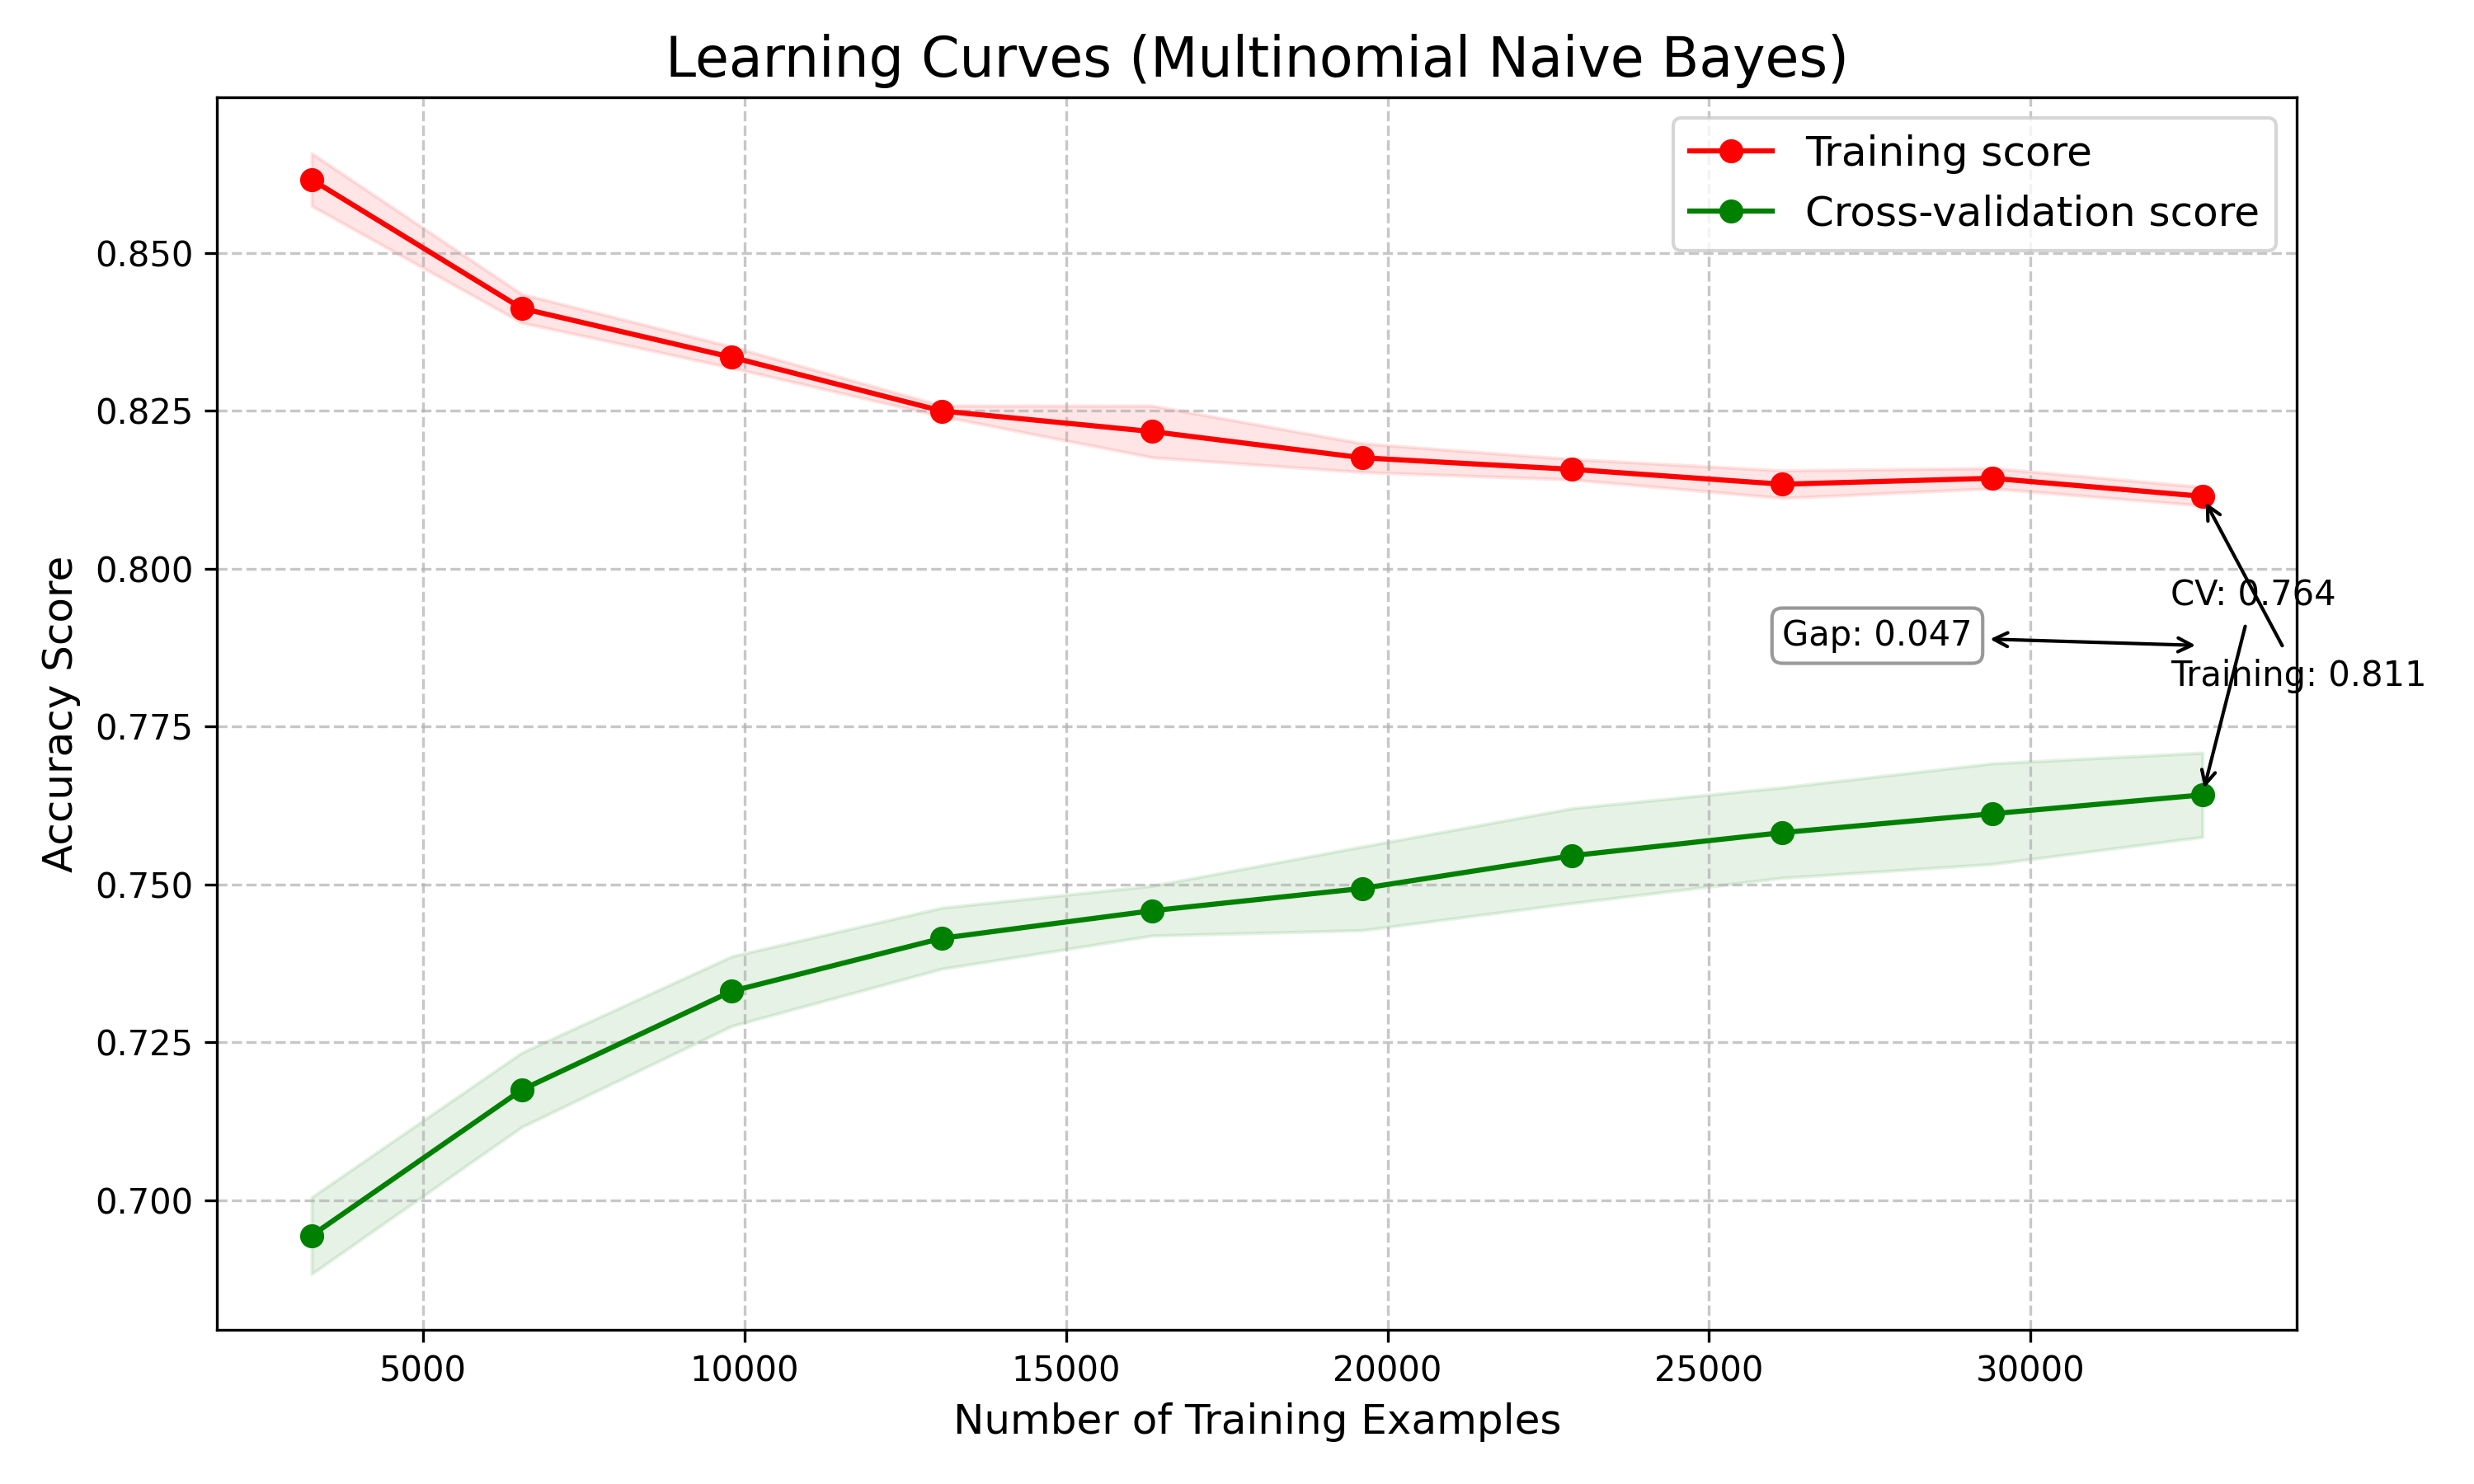
\includegraphics[width=0.9\columnwidth]{plots/mnb_learning_curves.png}}
\caption{Learning curves for the Multinomial Naive Bayes classifier showing training and cross-validation scores as training data increases.}
\label{fig:mnb_learning}
\end{figure}

\subsection{Feature Representation Comparison}
The different feature extraction approaches had minimal impact on model performance, with all three methods achieving similar results:

\subsubsection{Count Vectorization (Naive Bayes)}
This approach provides a simple representation focusing on term frequency, which works well with the Naive Bayes probabilistic framework. It achieved the highest accuracy despite (or perhaps because of) its simplicity and was the most computationally efficient approach.

\subsubsection{TF-IDF Vectorization (SVM)}
TF-IDF provides a more sophisticated representation that emphasizes distinctive terms and downweights common terms that appear across many documents. The inclusion of n-grams (up to trigrams) did not provide substantial performance improvements despite moderate computational requirements. This approach may have contributed to overfitting (94.42\% training vs. 51.53\% validation accuracy) by creating a complex feature space that allowed the model to memorize training examples. The high-dimensional feature space created by n-grams likely led to the model finding spurious patterns that did not generalize.

\subsubsection{Contextual Embeddings (BERT)}
BERT represents a sophisticated deep learning approach that captures word meanings in context. Despite having a significantly more complex model architecture and the highest computational cost, it provided minimal performance benefit and performed slightly worse than the simplest approach (Naive Bayes).

These comparisons suggest that for this particular task, increased model complexity and more sophisticated feature representations do not translate to improved performance. The similar performance across all three approaches indicates that the challenge may lie in the inherent difficulty of distinguishing genres solely through lyrical content, rather than in the choice of classification algorithm or feature representation.

\subsection{Computational Considerations}
Given the similar performance across all models, computational efficiency becomes an important consideration:

\subsubsection{Multinomial Naive Bayes}
The Multinomial Naive Bayes model features the fastest training and prediction times (seconds), minimal memory requirements (<100MB), and the simplest implementation and deployment. It achieved the best performance despite being the least complex of the three approaches.

\subsubsection{Support Vector Machine}
The SVM model requires moderate training time (minutes) and moderate memory requirements (100MB-1GB). It needs more hyperparameter tuning compared to Naive Bayes and delivered performance slightly below Naive Bayes despite its greater complexity.

\subsubsection{BERT}
BERT demands significant training time (hours on GPU) and substantial memory requirements (several GB). It requires specialized hardware (GPU) for efficient training and is the most difficult to deploy in resource-constrained environments. Despite being the most complex and computationally expensive approach, it achieved the lowest accuracy among the three models.

These results highlight that for this particular task, the simplest and most computationally efficient approach (Multinomial Naive Bayes) not only performed the best but also required the least resources. This observation challenges the common assumption that more complex models necessarily yield better results and suggests that model selection should carefully consider the trade-off between performance and computational efficiency.

\subsection{Accuracy Comparison}
Fig. \ref{fig:accuracy_comparison} presents a comparison of the accuracy achieved by all three classification methods on the validation dataset. The Multinomial Naive Bayes model achieved the highest accuracy at 52.39\%, slightly outperforming both the SVM (51.53\%) and BERT (51.49\%) models. The minimal differences between these approaches suggest that the task of genre classification based solely on lyrics remains challenging, with all models performing only marginally better than random chance.

\begin{figure}[htbp]
\centerline{\includegraphics[width=0.9\columnwidth]{plots/accuracy_comparison.png}}
\caption{Comparison of model accuracies: Multinomial Naive Bayes (52.39\%), SVM (51.53\%), and BERT (51.49\%) on the validation dataset.}
\label{fig:accuracy_comparison}
\end{figure}

\section{Conclusion}
This study demonstrates that genre classification of lyrics presents significant challenges, with all three models achieving accuracies only slightly above chance level. As illustrated in Fig. \ref{fig:accuracy_comparison}, the Multinomial Naive Bayes classifier achieved the highest accuracy at 52.39\%, followed closely by SVM (51.53\%) and BERT (51.49\%). These results suggest that lyrical content alone may not contain sufficient genre-specific signals for robust classification, or that the distinction between Pop and Rap/Hip-Hop lyrics may be more subtle than initially anticipated.

The results show that:
\begin{enumerate}
\item Traditional machine learning approaches like Multinomial Naive Bayes perform competitively with or slightly better than more complex models for this task
\item The inclusion of advanced features such as TF-IDF weighting, n-grams, and contextual embeddings did not significantly improve classification accuracy
\item All models perform only marginally better than random chance, highlighting the challenging nature of genre classification based solely on lyrics
\item The computational efficiency of simpler models may make them preferable when performance differences are minimal
\item The SVM model exhibited severe overfitting (94.42\% training accuracy vs. 51.53\% validation accuracy), demonstrating that complex models can excel at memorizing training data without capturing generalizable patterns
\end{enumerate}

The confusion matrices (Fig. \ref{fig:mnb_confusion} and Fig. \ref{fig:svm_confusion}) demonstrate the difficulty all models faced in clearly distinguishing between genres, suggesting substantial overlap in vocabulary and content between Pop and Rap/Hip-Hop lyrics.

Future work could explore multimodal approaches that combine lyrics with audio features, more fine-grained genre classifications, or the development of more specialized features tailored specifically to capture genre-distinctive patterns in lyrics. The learning curves (Fig. \ref{fig:mnb_learning}) suggest that additional training data alone might not significantly improve model performance without more fundamental improvements to feature engineering or classification approaches. Despite the challenges, this study provides valuable insights into the limitations of text-based genre classification and establishes important baselines for future research in this area.

\begin{thebibliography}{00}
\bibitem{tzanetakis2002musical} G. Tzanetakis and P. Cook, ``Musical genre classification of audio signals,'' IEEE Transactions on Speech and Audio Processing, vol. 10, no. 5, pp. 293-302, Jul 2002.
\bibitem{lidy2005evaluation} T. Lidy and A. Rauber, ``Evaluation of feature extractors and psycho-acoustic transformations for music genre classification,'' in Proc. 6th Int. Conf. Music Information Retrieval, 2005, pp. 34-41.
\bibitem{choi2017convolutional} K. Choi, G. Fazekas, M. Sandler, and K. Cho, ``Convolutional recurrent neural networks for music classification,'' in 2017 IEEE International Conference on Acoustics, Speech and Signal Processing (ICASSP), 2017, pp. 2392-2396.
\bibitem{fell2014lyrics} M. Fell and C. Sporleder, ``Lyrics-based analysis and classification of music,'' in Proceedings of COLING 2014, the 25th International Conference on Computational Linguistics: Technical Papers, 2014, pp. 620-631.
\bibitem{mayer2008rhyme} R. Mayer, R. Neumayer, and A. Rauber, ``Rhyme and style features for musical genre classification by song lyrics,'' in Proc. 9th Int. Conf. Music Information Retrieval, 2008, pp. 337-342.
\bibitem{mccallum1998comparison} A. McCallum and K. Nigam, ``A comparison of event models for naive bayes text classification,'' in AAAI-98 Workshop on Learning for Text Categorization, 1998, pp. 41-48.
\bibitem{kim2014convolutional} Y. Kim, ``Convolutional neural networks for sentence classification,'' in Proceedings of the 2014 Conference on Empirical Methods in Natural Language Processing (EMNLP), 2014, pp. 1746-1751.
\bibitem{sebastiani2002machine} F. Sebastiani, ``Machine learning in automated text categorization,'' ACM Computing Surveys, vol. 34, no. 1, pp. 1-47, 2002.
\bibitem{mikolov2013distributed} T. Mikolov, I. Sutskever, K. Chen, G. Corrado, and J. Dean, ``Distributed representations of words and phrases and their compositionality,'' in Advances in Neural Information Processing Systems 26, 2013, pp. 3111-3119.
\bibitem{devlin2018bert} J. Devlin, M.-W. Chang, K. Lee, and K. Toutanova, ``BERT: Pre-training of deep bidirectional transformers for language understanding,'' arXiv preprint arXiv:1810.04805, 2018.
\bibitem{logan2004semantic} B. Logan, A. Kositsky, and P. Moreno, ``Semantic analysis of song lyrics,'' in 2004 IEEE International Conference on Multimedia and Expo (ICME), 2004, pp. 827-830.
\bibitem{hu2010improving} Y. Hu and J. S. Downie, ``Improving mood classification in music digital libraries by combining lyrics and audio,'' in Proc. 10th Annual Joint Conference on Digital Libraries, 2010, pp. 159-168.
\end{thebibliography}

\end{document} 